\documentclass[a4paper,12pt]{article}
\usepackage{amssymb}
\usepackage{amsfonts}

% Кодировка и язык
\usepackage[utf8]{inputenc}
\usepackage[T2A]{fontenc}
\usepackage[russian]{babel}


% Математические пакеты
\usepackage{amsmath,amsfonts,amssymb}
%Таблицы
\usepackage{array}
\usepackage{booktabs} % Для более красивых горизонтальных линий в таблицах
\usepackage{graphicx}
\usepackage{array}
\usepackage{booktabs}
% Геометрия страницы
\usepackage{geometry}
\geometry{top=2cm, bottom=2cm, left=2.5cm, right=2.5cm}
% Гиперссылки (лучше загружать последним)
\usepackage{hyperref}


% Настройки заголовка
\title{Домашнее задание}
\author{Студент: \textbf{Ростислав Лохов}}
\date{\today}

\begin{document}

% Титульный лист
\begin{titlepage}
    \centering
    \vspace*{1cm}

    \Huge
    \textbf{Домашнее задание}

    \vspace{0.5cm}
    \LARGE
    По курсу: \textbf{Экономика}

    \vspace{1.5cm}

    \textbf{Студент: Ростислав Лохов}

    \vfill

    \Large
    АНО ВО Центральный университет\\
    \vspace{0.3cm}
    \today

\end{titlepage}

% Содержание
\tableofcontents
\newpage

% Основной текст
\section{Сине-Красный уровень}


\subsection{Задача 1}
Средний продукт труда - кол-во произведенной продукции, которое в среднем приходится на одного человека
Предельный продукт труда - изменение кол-ва произведенной продукции, которое связано с наймом дополнительного работника.
Средние переменные издержки - переменные издержки, которые в среднем приходятся на одну единицу выпущенной продукции.

Тогда предельные переменные издержки - отношение заработной платы к предельному продукту труда = $0.5$
Средние переменные издержки - отношение ставки заработной платы к среднему продукту труда = $0.33$

\subsection{Задача 2}
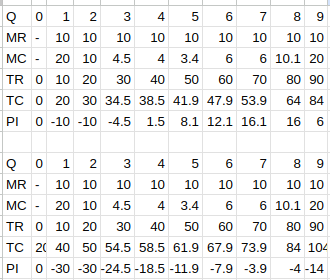
\includegraphics[scale=0.55]{graphs/6.1.png}


\subsection{Задача 3}
\begin{enumerate}
    \item Производство ПО (Разработка дорогая, копирование дешёвое) - Положительная(Jetbrains)
    \item Крупные агрохолдинги (Сложно управлять землёй, ограниченность) - Отрицательаня
\end{enumerate}

\subsection{Задача 4}
\begin{enumerate}
    \item Утопленные: Логистические центры(специализированные под конкретную задачу и трудно перепродать т.к рынок только развивается), ПО и технологии (уникальные, не для других целей), Реклама(деньги уже потрачены)
    \item Постоянные: Аренда, управление, амортизация оборудования, страховка, коммуналка
    \item Почему не нарастили клиентскую базу - Рынок был не готов, предложение не ценно
    \item Высокие постоянные издержки, низкая выручка, Точка безубыточности очень далеко(нужен огромный обьем), Большие издержки и маленькая выручка не позволили достичь прибыльности
    \item Дотком - от слова .com Пузырь доткомов - спекулятивный пузырь, завышенные оценки интернет компаний
    \item Эйфория вокруг интернета, переоценка перспектив, фокус на росте, не на прибыли, легкие инвестиции.
\end{enumerate}

\subsection{Задача 5}
\begin{enumerate}
    \item Авиабилеты - предельные затраты на одного пассажира низкие(динамическое ценообразование)
    \item Фитнес клубы - Высокие постоянные затраты на помещение и оборудование, предельные затраты на клиента в непиковое время - низкие
    \item Онлайн образование - высокие затраты на платформу и создание курсов, предельные затраты на одного обучающегося - низкие
    \item Облачные сервисы - огромные затраты на инфраструктуру, предельные затраты на нового клиента - минимальны.
\end{enumerate}

\section{Черный уровень}
\subsection{Задача 1}
\begin{enumerate}
    \item $MP_L = \frac{\Delta TP}{\Delta L} = \alpha K^{\beta}L^{\alpha - 1}$ $MPL > 0 $ т.к всё > 0
    \item $\Delta^2 = a(a-1)L^{a-2}K^b<0$ значит MPL убывает
    \item Аналогично с MPK: $\Delta = bL^aK^{b-1}>0$ $\Delta^2 = b(b-1)(L^aK^{b-2})<0$
    \item $\ln(TP)=a\ln(L)+b\ln(K)$
    \item $\delta \ln(TP) = a*0.01 \Rightarrow \Delta TP = a$
    \item $\delta \ln(TP) = b*0.01 \Rightarrow \Delta TP = b$
    \item $TP(tL, tK)=t^{a+b}L^aK^b$
\end{enumerate}

\subsection{Задача 2}
\begin{enumerate}
    \item $\delta TR = 12-1.8Q=0 \Rightarrow Q = 6\frac{2}{3}$ $P=6$ $TR_{max} = 40$
    \item $\pi = TR-TC \Rightarrow d\pi = 0.09Q^2+0.4Q-10=0 \Rightarrow Q = 8.56, P=4.3, \pi = 40.5$
\end{enumerate}


\begin{enumerate}
    \item С точки зрения математики всё корректно
    \item С точки зения издержек - функция кубическая, что-то очень большое
    \item Цена ниже издержек
    \item Оптимальные точки не совпадают
    \item Отрицательная прибыль
    \item Математически корректно, экономически некорректно
\end{enumerate}



\end{document}